\documentclass[conference]{IEEEtran}

\usepackage{graphicx}
\usepackage{amsmath}
\usepackage{url}

\ifCLASSINFOpdf
  % \usepackage[pdftex]{graphicx}
  % declare the path(s) where your graphic files are
  % \graphicspath{{../pdf/}{../jpeg/}}
  % and their extensions so you won't have to specify these with
  % every instance of \includegraphics
  % \DeclareGraphicsExtensions{.pdf,.jpeg,.png}
\else
  % or other class option (dvipsone, dvipdf, if not using dvips). graphicx
  % will default to the driver specified in the system graphics.cfg if no
  % driver is specified.
  % \usepackage[dvips]{graphicx}
  % declare the path(s) where your graphic files are
  % \graphicspath{{../eps/}}
  % and their extensions so you won't have to specify these with
  % every instance of \includegraphics
  % \DeclareGraphicsExtensions{.eps}
\fi

\begin{document}

\title{Machine Learning For Cognitive Radio}

\author{\IEEEauthorblockN{Afaque Hussain}
\IEEEauthorblockA{Department of Computer Science\\
University of Helsinki,\\
Finland.\\
Email: Afaque.Hussain@cs.helsinki.fi}}

% make the title area
\maketitle

% As a general rule, do not put math, special symbols or citations
% in the abstract
\begin{abstract}
A Cognitive Radio (CR) is a radio which learns from its operating environment and adapts itself so as to optimize its performance. Learning and adaptation abilities can be imparted to a radio using various techniques present in the field of Artificial Intelligence. In this paper, we will discuss some of the Artificial Intelligence techniques, namely, Artificial Neural Networks (ANN), Meta-heuristics algorithms such as Genetic Algorithms (GA), Simulated Annealing (SA) etc, Hidden Markov Models (HMM), Rule Based Systems (RBS), Case Based Systems (CBS) and Ontology Based Systems (OBS). We will discuss their strengths, drawbacks and their application to Cognitive Radio. We will also discuss the problem of controlling the outcome of a system where intelligent systems work together, interact and collectively try to achieve a specified goal. In the end, we will see some practical implementations of a Cognitive Radio followed by its challenges.
\end{abstract}

% For peer review papers, you can put extra information on the cover
% page as needed:
% \ifCLASSOPTIONpeerreview
% \begin{center} \bfseries EDICS Category: 3-BBND \end{center}
% \fi
%
% For peerreview papers, this IEEEtran command inserts a page break and
% creates the second title. It will be ignored for other modes.
\IEEEpeerreviewmaketitle



\section{Introduction}
% no \IEEEPARstart
    Studies around the world have confirmed that the radio frequency spectrum is not being efficiently utilized \cite{1}. In some parts of the world, all the available radio frequencies are licensed to either corporate organizations or government bodies leading to a situation called ``Spectrum Drought". Among these licensed radio frequencies, some frequencies have a very high traffic while few frequencies are rarely being used. For example, the frequencies used by cellular networks are found to be highly congested with traffic while the frequencies reserved for military operations are not fully utilized to their potential. Moreover, the usage of a particular frequency varies according to a given time and place. The user to whom the channel is assigned is called as a `Primary User' while other users are called as `Secondary Users'. To efficiently utilize the radio frequency spectrum, secondary users must be allowed to use a channel assigned to a primary user, provided that they do not interfere with the transmission of the primary users. This requires dynamic configuration and adaptation of a radio in response to dynamic radio environments and changing Quality of Service (QoS) requirements.

	Cognitive Radio attempts to solve this problem by sensing and adapting to its environment. A Cognitive Radio is basically a transceiver which senses the wireless spectrum and adjusts the radio parameters to use the spectrum efficiently. An example of a Cognitive Radio is IEEE 802.11 modulation controller which switches from 16 Quadrature amplitude modulation to Quaternary phase shift keying to binary phase shift keying as signal to noise ratio decreases \cite{4}. A Cognitive Radio is able to perceive and understand the environment in which it is operating, take decisions, reconfigure the radio according to the decisions taken after reasoning and learning the impact of these decisions on the performance of the radio. All these attributes namely, observation, reconfiguration and cognition can be encapsulated into a single component called ``Cognition Engine". While a normal radio would not suffice for the requirements of implementing a Cognitive Radio, a more configurable radio called `Software Defined Radio' (SDR) is developed. A SDR is a programmable radio in which the components such as amplifier, modulator, mixers, etc. have been implemented as a software. A SDR is usually implemented using embedded systems or a personal computer. Incorporating cognition to a SDR transforms it into a Cognitive Radio. According to the researchers of Virginia Tech, a Cognitive Radio is a ``Software Defined Radio with a Cognitive Engine (CE) brain" \cite{5}. The first phone call using Cognitive Radios was made on January 11, 2010 in Center for Wireless Communication (CWC) at University of Oulu over Cognitive Radio Assisted Mobile Ad-Hoc Network developed by CWC researchers \cite{2}.
    
    In this paper, we discuss various artificial intelligence techniques which impart intelligence to a radio. Section II explores the architecture of a Cognitive Radio, reasoning and planning in a Cognitive Engine followed by a discussion on various artificial intelligence models in Section III. In Section IV, we discuss the implementation of a Cognitive Engine using appropriate artificial intelligence models. In Section V, we discuss the application of Game Theory to Cognitive Radio followed by a discussion on practical implementations of Cognitive Radio in Section VI. We briefly discuss the challenges of Cognitive Radio in Section VII and finally conclude the paper with our final remarks in conclusion.

\section{Reasoning and Planning}

Machine Learning deals with the study and implementation of systems which learn from data. Before we go into the details of how reasoning and learning can be implemented, we will look at the architecture of a Cognitive Radio.

\subsection{Architecture of a Cognitive Radio}
As mentioned previously, a Cognitive Radio can be thought as an extension to a Software Defined Radio with a Cognitive Engine. Figure \ref{fig_arch} shows a general architecture of a Cognitive Radio.


\begin{figure}[!t]
\centering
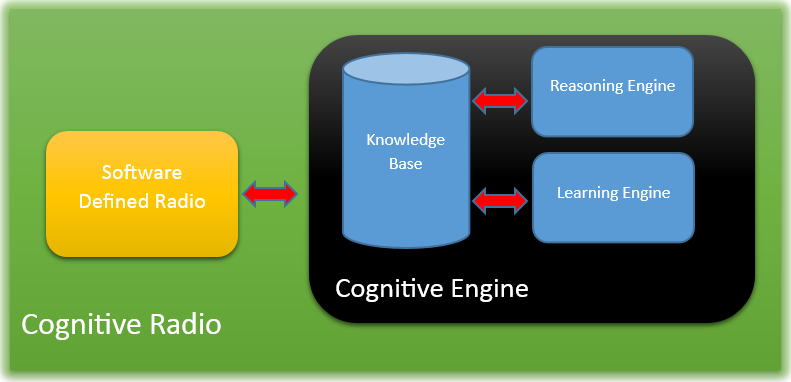
\includegraphics[width=3.5in]{Figure_1}
\caption{Architecture of Cognitive Radio.}
\label{fig_arch}
\end{figure}

	A Cognitive Engine consists of a Knowledge Base, a reasoning engine and a learning engine \cite{4}. They collectively impart intelligence to a Software Defined Radio. A Knowledge Base consists of information, using which a Cognitive Radio generates conclusions. The reasoning engine does the ``thinking" or derives conclusions based on the information stored in the Knowledge Base. The learning engine updates the Knowledge Base according to the lessons learned by observing the impact of the actions taken by a Cognitive Radio.

\subsection{Reasoning}
In this section, we will discus how a reasoning engine functions in a Cognitive Radio. As mentioned earlier, a Cognitive Engine consists of a Knowledge Base according to which the reasoning engine takes decisions. A Knowledge Base generally consists of two data structures. The first data structure is a set of predicates, which are logical expressions representing the current environment state. Below is an example of a simple predicate, which can either be evaluated to true or false:
\begin{equation}
\centering
\label{A predicate}
\alpha  \wedge  \beta.
\end{equation}
The second data structure is a set of actions. These actions represent the operations that a reasoning engine could perform to change the state of operation of a Cognitive Radio in response to changing radio environments. Each action has a set of preconditions and post-conditions. Actions are performed only when preconditions are evaluated to be true. Post conditions represent the state of the Knowledge Base after the action has been taken \cite{4}.
	
	Let us take an example to better understand these concepts. Consider a Cognitive radio that has been defined an objective to decrease the modulation rate as the Signal to Noise Ratio (SNR) decreases. Following predicate: 
	
\begin{equation}
\centering
modRate(QPSK) \wedge snr(5 dB).
\end{equation}
and following action:
\begin{equation}
\begin{split}
& action:decreaseModulationRate  \\
& precondition:modRate(QPSK) \wedge snr(\leq8dB) \\
& postcondition:\neg modRate(QPSK)	 \wedge modRate(BPSK). \\
\end{split}
\end{equation}
will be stored in the Knowledge Base \cite{4}.

When SNR decreases below 8 dB, decreaseModulationRate action will be executed by the reasoning engine and post condition is applied as a result of which modulation changes from QPSK to BPSK.

	At any given instance of time, the reasoning engine senses the current environment and determines appropriate action needed to be performed. It evaluates all the resulting states generated by all possible actions and selects the most optimal state according an objective function. An objective function represents the overall goal of a Cognitive Radio. It is possible that we could program all the actions into a Cognitive Radio, but in complex environments, a large amount of actions would be needed to be programmed for all possible states. Hence, there is a need for learning engine which would auto-generate the required actions based on its previous experience.

\subsection{Learning}
	A learning engine makes modification to a Knowledge Base according to what it learns during the learning process. A learning engine aims to model a partially known environment as accurately as possible so that a Cognitive Radio can adapt and operate optimally and tries to determine which input state will maximize a defined objective function. There is no explicit mathematical relation between the input states and the objective function, which makes the task of implementing a learning engine difficult \cite{4}. However, a learning engine can be implemented using one of many learning algorithms available such as Artificial Neural Networks, Hidden Markov Models, Genetic Algorithms etc. which we will discuss in the next section.


\section{Artificial Intelligence models}
	Implementing a Cognitive Engine is an active area of research. There are vast array of artificial intelligence techniques available which could be used to implement different components of a Cognitive Engine. In this section we will explore various artificial intelligence techniques, their strengths, their limitations and their application to Cognitive Radio.

\subsection{Artificial Neural Network (ANN)}
	ANN is perhaps the oldest artificial intelligence technique with over six decades of research being carried in this field. Inspired by the biological neurons and nervous system, ANN is adaptable to the type of problem it is solving. ANN is used in a wide variety of fields to solve many real world problems. 
    
    ANN is a mathematical model which consists of interconnected group of artificial neurons \cite{6}. An artificial neuron consists of two or more weighted inputs and a single output. A function called as activation function is defined for each artificial neuron which sums up the weighed inputs to a neuron and decides whether the neuron should be activated or not. If a neuron is activated, then a signal is a sent from the output of a neuron which may act as an input to many other neurons in an ANN. The network between these artificial neurons is not static, it changes according to the type of problem an ANN is solving. 
    
    Figure \ref{fig_ann} shows a simple ANN. In this type of a network, there is a layer of input neurons, a layer of output neurons and an intermediate layer of neurons which form connections with other neurons in a such way so as to produce a signal flow as desired by the problem given to an ANN. An ANN is trained using various learning techniques such as supervised learning, unsupervised learning and reinforcement learning. Algorithms are designed to alter the weights and connections between the neurons. Hence, during a learning procedure of an ANN, the neurons form a dynamic network to solve a given problem. 

\begin{figure}[!t]
\centering
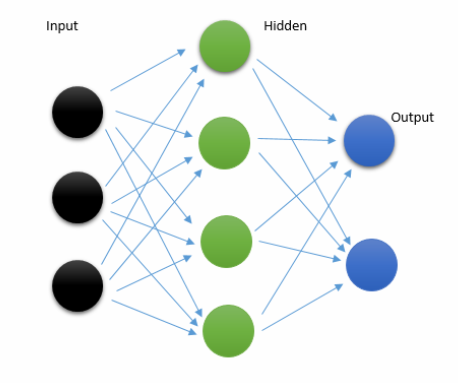
\includegraphics[width=3.5in]{Figure_2}
\caption{Artificial Neural Network.}
\label{fig_ann}
\end{figure}
    
    ANN has a remarkable ability to dynamically adapt and learn patterns of a system. It does not need to be explicitly programmed and can be trained at any time. Based on observation, ANN can infer a function due to which it has applications in solution of many real world problems such as function approximations, classification, data processing and robotics. ANN can be used in classification of radio frequency spectrum and adaptation of a Cognitive Radio to dynamic environments. ANN can be constructed and trained in such a way that it is able to infer properties of a partially known environment. For example, consider Figure 3, in which the input to an ANN is SNR, received frames, erroneous frames and idle time. Using these input values an ANN is able to characterize the performance of a network by providing information such as throughput, delay and reliability. Analytical models can do an equally well job for such a task but analytical models have scalability problems. It is relatively easy to add an extra parameter as an input to an ANN than to make the corresponding changes in analytical models. 

    Authors of \cite{8} develop a Multi-Layered Feed Forward Neural Network (MFNN) for real time communication performance characterization of a Cognitive Radio based on the measurements carried out by the device itself. The design of a MFNN is shown in Figure 3. The network is trained using supervised learning. For characterization of throughput performance of an infra structured 802.11 cell, the information regarding the number of users is required. But this information is not usually available to a Cognitive Radio. Hence, an ANN uses environmental features such as SNR, received frames and erroneous frames to characterize the throughput of a 802.11 cell. The values predicted by the this designed ANN are very close to the values predicted by Bianchi's model which takes into account the actual number of users.

    Detecting unused bands without interfering with the primary user's communication is a challenging area of research. Authors of \cite{7} apply ANN for signal classification in conjunction with cyclic spectral correlation for both the cases, where information regarding the carriers' signal and band-with is available and information regarding the carriers' signal and band-with is not available. Authors of \cite{7} propose that prepossessing of a signal be done using cyclic spectral correlation and then classification of the output generated by the previous step be done using ANN.  
    
\begin{figure}[!t]
\centering
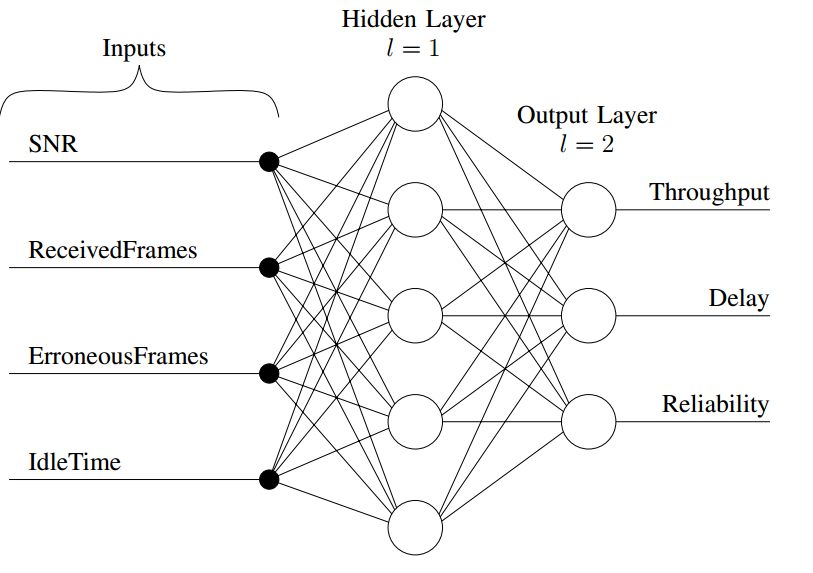
\includegraphics[width=3.5in]{Figure_3}
\caption{Performance Characterization using Artificial Neural Networks \cite{8}.}
\label{fig_ann2}
\end{figure}
	

\subsection{Meta-heuristic Algorithms}
	 Implementing a learning engine is a challenging task as there is no apparent and easily discovered relationship between the input states and an objective function. Consider for example the problem of parameter optimization of a Cognitive Radio, a Cognitive Radio has to find an optimal set of parameters for a given radio environment. This problem boils down to the task of searching a set of parameters from a large search space. The most optimal solution is to use the brute force technique but it is impractical to implement as it takes unacceptably long time to search. Meta-heuristic algorithms can be used to solve such problems which try to find a solution under acceptable time at the expense of optimality. Meta-heuristic algorithms use a technique in which they modify candidate solutions to find near optimal solutions with respect to given objective levels. Hence, meta-heuristic algorithms are an ideal solution for implementing a learning engine, using which a Cognitive Radio can fine tune its parameters according to the required performance metrics. We will discuss few meta-heuristic algorithms which are important from the perspective of a Cognitive Radio. 

\subsubsection{Genetic Algorithms}
	Genetic Algorithm is a search heuristic which belongs to a class of evolutionary algorithms that derive their inspiration from the evolution process of life and natural selection of species \cite{6}. In this algorithm, a random set of candidate solutions are selected which are denoted as `chromosomes'. The overall objective of the algorithm is formulated as a fitness function. The chromosomes are evaluated against the fitness function and candidates which meet the requirements set by the fitness function are selected. Using these selected chromosomes, new population is created by either combining them or by a process called mutation. Several such evaluations lead to a generation and several generations lead to desired result. Genetic Algorithms produce solutions which are very close to the optimal solution but they might take a long time to converge to a result.

    Newman et al. use Genetic Algorithms for solving the parameter optimization problem \cite{9}. They also address the problem of reducing the convergence time of a genetic algorithm. They use the available information about a given environment and seed a genetic algorithm with a good set of chromosomes which are much likely to lead to an optimal solution. Such techniques improve the time to find a solution by 480\% over normal genetic algorithm.
    
    Kim et al. use Genetic Algorithm for dynamic spectrum management \cite{10}. They try to address the problem of maximizing the spectral efficiency while minimizing the interference with primary users. A two step Genetic Algorithm is used to prevent the biasing of dominant parameter in the optimization process. Two functional blocks are used in which one performs channel selection and other performs transmitter parameter selection. They implement a software testbed using a two step Genetic Algorithm. Simulation results show that such a Cognitive Radio selects optimal parameters in a given radio environment. 
    
	
\subsubsection{Simulated Annealing}
	Simulated Annealing is a meta-heuristic algorithm which tries to find an approximate global optimum in a large search space. It takes inspiration from the annealing process in metallurgy where the metal is first heated and then cooled in a controlled way so as to decrease its defects. Similarly, in this algorithm, initially the probability of accepting worse solutions is kept high. With the passage of time, the probability of accepting worse solution is decreased so as to converge to an optimal solution. Keeping the initial window of worse solution wide enables an in-depth search of the search space. For example, consider the problem of finding a global optimum as shown in Figure 4. Initially, the algorithm wanders around the local optimums to find an optimum solution. With the passage of time, as the probability of accepting worse solution decreases, the algorithm wanders in a very small space near the global optimum and eventually finds a global optimum. 

\begin{figure}[!t]
\centering
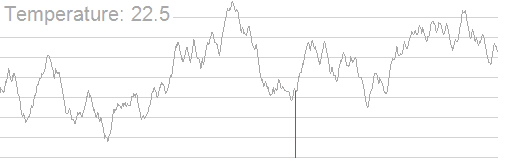
\includegraphics[width=3.5in]{Figure_4}
\caption{Searching global optimum using Simulated Annealing \cite{23}.}
\label{fig_sa}
\end{figure}

In \cite{11}, Kaur et al. use Simulated Annealing for solving the problem of finding a set optimum parameters for a Cognitive Radio to minimize power consumption, minimize bit error rate, maximize throughput, minimize interference and maximize spectral efficiency. The authors carry out simulation for a single carrier Cognitive Radio using Simulated Annealing and the compare the results with a Genetic Algorithm solution for the same problem. Comparison results show that Simulated Annealing finds more optimal solutions than a Genetic Algorithm solution but takes a longer time and more number of iterations to find an optimum solution than a Genetic Algorithm solution.

\subsubsection{Tabu search}
	Local search heuristics take a candidate solution and try to find a similar solution which differs with the chosen candidate solution in few minor details in hope to find a more improved solution. Local search algorithms have a drawback that they get stuck in sub-optimal solutions. Tabu search enhances the performance of these local searches by maintaining a memory structure called `Tabu' (forbidden). This prevents the algorithm from visiting the same solution more than once and prevents it from being stuck in sub-optimal solutions. 
    
    In \cite{12}, Subramanian et al. use Tabu search algorithm for centralized channel assignment problem with an objective of minimizing the overall network interference. Subramanian et al. solve the centralized channel assignment in two phases. In the first phase, Tabu search algorithm is initiated where a random assignment takes place and these candidate solutions are improved with an objective of minimizing the network interference. For a fast convergence to a solution, a Tabu list is maintained, such that reassignment of a channel to a same communication link is avoided. The algorithm terminates when a set number of iterations haven taken place without improving a candidate solution. It might be possible that the solution yielded by the previous step might violate interface constraints. Interface constraint violations are prevented in the second phase by a procedure called `merging', which is detailed in \cite{12}.

\subsubsection{Ant colony optimization (ACO)}
	Inspired by the behavior of ants, ACO algorithm uses a similar approach as applied by the ants in finding an optimal path to their food source. Figure 5 outlines the approach of ants in finding the optimal route to the food source. As ants are blind, they wander randomly in search of food, leaving a trail of a particular chemical called `Pherome' along the path which they travel. Other ants follow these trails and over time, the optimal route becomes stronger as more ants travel through that path and less optimal routes get eliminated as pherome gets evaporated after certain period of time. In this way, the ants find an optimal route to their food. Similarly, ACO mimics the behaviour of ants to find a global optimal in a large search space \cite{6}.

\begin{figure}[!t]
\centering
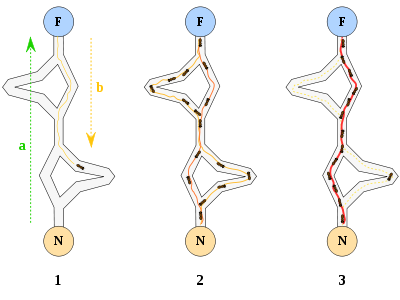
\includegraphics[width=3.5in]{Figure_5}
\caption{Optimal Path selection by Ants \cite{24}.}
\label{fig_aco}
\end{figure}

    Authors of \cite{13} apply an enhanced version of ACO algorithm  for dynamic channel assignment problem in Cognitive Radio Networks. The algorithm is initialized with various parameters required by the algorithm such as number of iterations the algorithm should run, number of primary users, pherome value, pherome evaporation rate etc. As the algorithm finds local optimums, it updates the pherome values simulating the creation of a pherome trail. The channel assignment results are obtained from the algorithm and compared with the overall objective function of the algorithm. The algorithm stops when it has iterated for a specified number of times and the best candidate solution which meets the objective function requirements is selected as the solution. Simulation results demonstrate that ACO performs well at the task of dynamic channel assignments which results in optimal performance of a Cognitive Radio Network.

\subsection{Hidden Markov Models (HMM)}
    HMM is used to model the behavior of a complex random phenomenon \cite{5}. A Markov process is a process whose future states can be predicted solely using its current state. HMM is a system model which models a Markov process whose states are hidden and only output is visible. HMM can be better understood with help of an example called the `Urn Problem'. Consider a room which is not visible to an outside person. The room contains `n' Urns (vases), each Urn having certain number of balls differentiated by their color. A genie present inside the room selects an Urn using some procedure, which is also unknown to the outside person. After selecting an Urn, the genie draws a ball randomly and places it on a conveyor belt, whose one end is visible to the outside person. A model which models such type of a process where the states of a process are hidden and only output is visible is called a Hidden Markov Model. Urn example has a striking similarity with the usage of a radio channel by its primary user. Hence, HMM can be used to model and predict the usage of a radio channel by its primary user so as to minimize the interference. HMM can also be used to train other learning algorithms such ANN, GA etc.

    Generally, secondary users sense a radio channel to see if it is being used by a primary user. This causes interference which results in degradation of performance of a primary user. Authors of \cite{14} use HMM to model and predict the spectrum occupancy of licensed radio bands. By predicting the spectrum holes and usage of the spectrum by primary users, a CR is able to efficiently utilize the spectrum while minimizing the interference. Authors of \cite{14} also develop a Markov-based Channel Prediction algorithm (MCPA) for dynamic spectrum allocation in Cognitive Radio Networks. Simulation results show that a MCPA based dynamic spectrum allocation produces improved throughput as compared to a Carrier Sense Multiple Access (CSMA) spectrum allocation technique. 

\subsection{Rule Based Systems}
	Rule Based Systems (RBS) are a way of storing and manipulating a knowledge base so that the information is interpreted in a useful way \cite{5}. A RBS consists of four basic components namely a rule base which consists of a list of rules, an inference engine which takes actions based on the inferred information from a rule base, a temporary memory and a user interface for input and output. RBS differ from procedural program in a way that it does not matter in which way the rules are executed unless all the rules are executed.

    Due to their simplicity, RBS can be used to implement a reasoning engine. However, the rule base should be complete and accurate for RBS to produce the desired results. In \cite{15}, Reed et al. design a rule based reasoning engine for a Cognitive Engine for IEEE 802.22 wireless rural area network. In \cite{4}, Clancy et al. develop a rule based reasoning engine using predicate calculus for enabling learning in the reasoning process.

\subsection{Ontology Based Systems}
	An ontology represents knowledge of a particular domain as a set of concepts and relationship between these concepts. An Ontology is used to reason about the properties of the objects of a given domain. An Ontology consists of classes, instances, attributes and relations as basic components. An ontology is used to model a particular domain and usually expressed using an ontology language \cite{3}.

    An ontology based system can logically deduce facts. An ontology based radio can logically deduce characteristics about itself and other radios. However, it might take a large amount of time to deduce these facts. In \cite{16}, Kokar et al. investigate Web Ontology Language for a Cognitive Radio and propose that a good ontology language should be able to express rules, introduce new functions and specify radio behaviors. In \cite{17}, Wang et al. use ontology based reasoning to implement self-awareness and interoperability between software defined radios. In \cite{18}, Poston et al. use ontology based reasoning to apply spectrum policy to dynamic spectrum access.

\subsection{Case Based Systems}
	Case Based Systems (CBS) attempt to solve problems by using the previous experiences of the problems solved. According to the authors of \cite{19}, a Case Based Reasoning (CBR) cycle consists of the following processes: 
\begin{enumerate}
\item Retrieve the most similar case.
\item Reuse the knowledge and information found in a similar case to solve the problem.
\item Revise the proposed solution.
\item Retain the parts of this experience which might be useful for future problem solving. 
\end{enumerate}

	By reusing the solution of similar cases and retaining certain parts of the solution for future use, the system is able to solve problems at a faster rate. However, the performance of this system is based on how previous cases are solved. If some of the cases were erroneously solved, then it is likely that these errors would propagate in future cases too. 

	CBS can be used to find a good solution in a given environment based on its previous experience in solving similar cases. In \cite{20}, Reed et al. design a Case Based Reasoning Cognitive Engine which obtains radio parameters for IEEE 802.22 WRAN application. Authors of \cite{21} design a Cognitive Engine using Case Based Reasoning and fuzzy logic for determining the channel type in WiMAX systems.
    
\section{Implementation of a Cognitive Engine}
    After the discussion of various artificial intelligence models, we will now look at how a Cognitive Engine can be implemented. As shown in Figure 6, ANN, Meta-heuristic algorithms such as GA, or HMM can be used to implement a learning engine. OBS, CBS and RBS are good at deducing information based on the contents of a knowledge base, hence they can be used to implement a reasoning engine and knowledge base. Appropriate models must be chosen to implement the components of a Cognitive Engine according to the requirements and objectives. 
    
    A SDR provides properties of a radio environment to a learning engine. Based on the input, the learning engine learns and models the environment. It then updates the knowledge base with the information learnt from a given environment. A reasoning engine picks up the information stored in a knowledge base, deduces new information and instructs a SDR the actions it needs to take so as to adapt itself to a given radio environment.

\begin{figure}[!t]
\centering
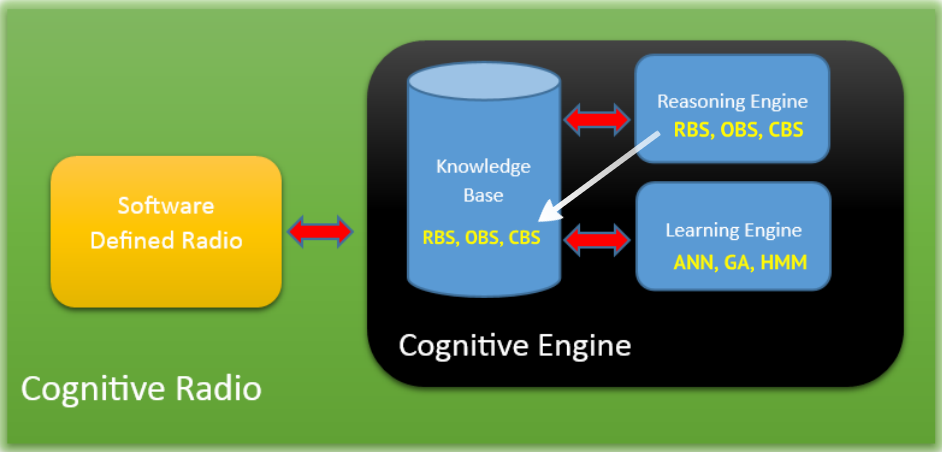
\includegraphics[width=3.5in]{Figure_6}
\caption{Implementation of a Cognitive Engine.}
\label{fig_ce}
\end{figure}

\section{Interaction of Intelligent agents}
	 We see that a Cognitive Engine cannot be implemented using a single artificial intelligence technique but rather each component can be implementing using a particular model which suits it accordingly. Whether we consider a Cognitive Radio as a single entity with Cognitive Engine or with a Cognitive Engine implemented with multiple artificial intelligence techniques, the overall outcome and performance is dependent on how various Cognitive Engines interact. There might be some cases where small changes in the network configuration could result in a chain reaction of Cognitive Engines, which may lead to an unlimited amount of adaptations. The adaptations may never converge and could make the network unstable.

	Therefore, designing artificial intelligence for a Cognitive Engine which considers its operation only in isolation would not suffice for the design of a Cognitive Radio, but they have to be designed in such a way that they take into account operation of other Cognitive Engines. The problem boils down to modeling how different networked intelligent agents interact. Game theory provides a collection of models which could predict the outcome of interaction of intelligent agents. The analogy between artificial intelligence in Cognitive Radio and human intelligence is so much that game theory is suggested to be applied for modeling the interaction of Cognitive Radios. By using various available game models to Cognitive Radio, researchers will be able to predict the outcome of various interacting Cognitive Radios and are able to control them so that all collectively accomplish a common goal. 

    Authors of \cite{22}, use potential games to model a Cognitive Radio Network to identify steady state conditions for the network. In game theory, potential games are characterized by a potential function which is a global function that expresses the change in strategy of players in that game. In the model constructed by the authors of \cite{22}, Cognitive Radios are players which take decisions according to a defined objective function. Network interference is set as the factor that influences the decision that Cognitive Radios take. A Cognitive Radio alters its power level or its waveform to minimize the interference it introduces in the network. Hence, using such a model, the authors develop potential functions which identify states such that interference introduced by the all the Cognitive Radios in a Cognitive Radio Network is minimum. 
	

\section{Practical Implementations}
	Researchers at Virginia Tech develop a proof of concept of a Cognitive Radio using Artificial Neural Networks called CoRTekS (Cognitive Radio Tektronix System) \cite{3}. It consists of a transmitter, a receiver and a personal computer on which a SDR and Cognitive Engine run. CoRTekS demonstrates the use of artificial intelligence techniques for parameter optimization of a Cognitive Radio. The Cognitive Engine of CoRTekS controls the transmitter and receiver by determining the best set of parameters according to the objective function defined. Test results show that CoRTekS selects a better set of parameters for a given radio environment by drawing relationship between these parameters and system performance. 

    Authors of \cite{4}, develop a Cognitive Radio using OSSIE, an open source software communications architecture core framework and Soar Cognitive Engine developed by University of Michigan. Given fixed power, frequency and bandwidth, the Cognitive Radio tries to select a modulation type and coding rate to maximize capacity in a Additive White Gaussian Noise (AWGN) channel and a non-AWGN channel. Simulation results show that the Cognitive Radio achieves optimal configuration of modulation and coding rate to efficiently utilize a given channel. 

\section{Challenges}
	With over a decade of research being carried in the field of Cognitive Radio, it could be said that this field is still in its infancy due to which practical implementation of Cognitive Radios still remains primary, basic and experimental. There is always a trade-off between complexity and performance. The more intelligent the Cognitive Engine is, the slower it is. In case of Artificial Neural Networks, a significant amount of learning samples are required to train the network before it performs at an optimal level. Hence, Cognitive Engines should be carefully designed keeping in mind the trade-offs between complexity and performance.
	
	Implementing Cognitive Engine is one thing, controlling the interaction of these intelligent entities is another challenge. All Cognitive Engines should be designed taking into account the interaction of other intelligent agents and should prevent infinite adaptations. Other issues such as fault tolerance, security etc. should also be addressed before Cognitive Radio becomes deploy-able in real world. \\


\section{Conclusion}
	We have seen in this paper, the application of various artificial intelligence techniques to a Software Defined Radio. We also discussed the strengths, drawbacks and application of these artificial intelligence models to a Cognitive Radio. We discussed the problem of modeling the interaction of intelligent systems. We also saw some elementary implementation of Cognitive Radios. However, we are far from creating a stable Cognitive Radio which can be deployed for real world use. Many problems, issues and challenges still need to be addressed, which provides a good platform for researchers of machine learning to apply the concepts of their field. 




% conference papers do not normally have an appendix


% use section* for acknowledgement
\section*{Acknowledgment}

I would like to thank Suzan Bayhan for helping me understand this topic and guiding me throughout the writing process of this paper. I also thank the reviewers of this paper for giving me feedback to further improve this paper.
% trigger a \newpage just before the given reference
% number - used to balance the columns on the last page
% adjust value as needed - may need to be readjusted if
% the document is modified later
%\IEEEtriggeratref{8}
% The "triggered" command can be changed if desired:
%\IEEEtriggercmd{\enlargethispage{-5in}}

% references section

% can use a bibliography generated by BibTeX as a .bbl file
% BibTeX documentation can be easily obtained at:
% http://www.ctan.org/tex-archive/biblio/bibtex/contrib/doc/
% The IEEEtran BibTeX style support page is at:
% http://www.michaelshell.org/tex/ieeetran/bibtex/
\bibliographystyle{IEEEtran}
% argument is your BibTeX string definitions and bibliography database(s)
\bibliography{ZedBib}
%
% <OR> manually copy in the resultant .bbl file
% set second argument of \begin to the number of references
% (used to reserve space for the reference number labels box)
%\begin{thebibliography}{1}

%\bibitem{IEEEhowto:kopka}
%H.~Kopka and P.~W. Daly, \emph{A Guide to \LaTeX}, 3rd~ed.\hskip 1em plus
%  0.5em minus 0.4em\relax Harlow, England: Addison-Wesley, 1999.
%\end{thebibliography}




% that's all folks
\end{document}

